\documentclass{beamer}

\usetheme{CambridgeUS}

\usepackage{amsmath}
\usepackage{graphicx}
\usepackage{tfrupee}

% FOR TABLE (according to table generated by ssconvert)
\def\inputGnumericTable{}
\usepackage[latin1]{inputenc}
\usepackage{color}
\usepackage{array}
\usepackage{longtable}
\usepackage{calc}
\usepackage{multirow}
\usepackage{hhline}
\usepackage{ifthen}
\usepackage{lscape}

\providecommand{\pr}[1]{\ensuremath{\Pr\left(#1\right)}}

\title{Assignment 6 \\ Papoulis Example 4.23}
\author{Kartheek Tammana}
\date{\today}
\logo{\large \LaTeX{}}

\begin{document}

\begin{frame}
    \titlepage
\end{frame}

\logo{}

\begin{frame}{Outline}
    \tableofcontents
\end{frame}

\section{Question}
\begin{frame}{Question}
    Over a period of 12 hours, 180 calls are made at random. What is the probability that in a 4
    hour interval, the number of calls is between 50 and 70?
\end{frame}

\section{Answer}
\begin{frame}{Variables}
    Let the Bernoulli variable $X \in \{0, 1\}$ denote whether a call lies within the 4 hour
    interval with $p_X(1) = p = 1 - q$.

    Let $Y \in \{0, 1, ... 180\}$ denote the number of calls in the four hour interval.

    $Y$ represents 180 trials of $X$.
\end{frame}

\section{Calculations}
\begin{frame}{Calculations}
    The probability that a single call in the 12 hour interval lies in the 4 hour interval
    is

    \begin{equation}
        p_X(1) = p = \frac{4 hr}{12 hr} = \frac{1}{3}
    \end{equation}

    Since $Y$ is a binomial variable, we have that,
    \begin{align}
        p_Y(k) &= \binom{180}{k} p^{k} q^{180-k} \\
               &= \binom{180}{k} \left(\frac{1}{3}\right)^{k} \left(\frac{2}{3}\right)^{180-k}
    \end{align}
\end{frame}

\begin{frame}
    We need to find
    \begin{align}
        \pr{50 \leq Y \leq 70} &= \sum_{k=50}^{70} p_Y(k) \\
        &= \sum_{k=50}^{70} \binom{180}{k} \left(\frac{1}{3}\right)^{k}
            \left(\frac{2}{3}\right)^{180-k} \\
        &\approx 0.9025098...
    \end{align}
    So we have that the required probability, that the number of calls in the interval is
    between 50 and 70, is approximately 0.9025.
\end{frame}

\section{Graph}
\begin{frame}{Graph}
    \begin{figure}[!ht]
        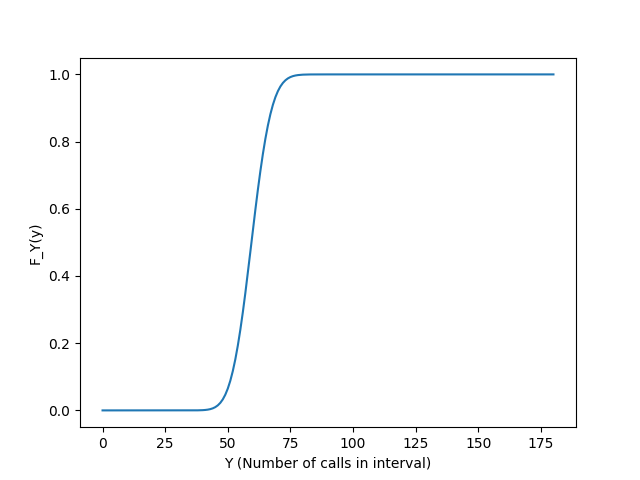
\includegraphics[width=\textheight]{figs/cdf.png}
        \caption{Cumulative Probability Function}
        \label{figure:1}
    \end{figure}
\end{frame}

\end{document}
